\chapter{Vertexing Search}

\section{Data and Monte Carlo Samples}
All of the events of interest (tridents, heavy photons, and wide-angle bremsstrahlung) are generated using MadGraph/MadEvent version 4 \cite{alwall_madgraph_2007}.
Background

\subsection{Data Processing and Normalization}

\subsection{Trident and Wide-Angle Bremsstrahlung Monte Carlo}
The background 

\subsection{Heavy Photon Monte Carlo}
\label{sec:ap_mc}
Heavy photon Monte Carlo is generated at values of $m_{A'}$ spaced out across the region of interest: 15, 16, 17, 18, 19, 20, 22, 24, 26, 28, 30, 35, 40, 50, 60, 70, 80, and 90 MeV.
In order to get complete coverage of $z>z_{target}$ for the purposes of the vertexing analysis, the decay vertices were displaced (in the direction of the heavy photon momentum, and accounting for variations in $\gamma$) according to an arbitrary decay length of $c\tau=1$ mm.

\section{Event Selection}
require layer 1

\section{Inputs}
The events passing cuts are reduced to a 2-D dataset of points $(m,z)$, where each point is the mass $m$ and vertex Z-coordinate $z$ of an event.




To test for a heavy photon at mass $m_{A'}$ and coupling $\epsilon^2$:

The dataset is cut to keep only events with $|m-m_{A'}|<1.4 \sigma_m(m_{A'},z)$.
This mass window is chosen to accept a large fraction of the signal events, without accepting too many background events.
A window of $\pm1.4\sigma$ optimizes significance for high-statistics, high-background experiments where significance is proportional to $S/\sqrt{B}$; it is not 
The mass resolution depends on the mass and the vertex position, and is estimated using Monte Carlo: this is explained in Section \ref{sec:mres}.

After cutting on $m$, the dataset is reduced to one dimension.
An additional cut is made to keep only events with $z>z_{cut}$, rejecting the region where the background strongly dominates and there is no sensitivity to a signal.

The events are assumed to be drawn from the sum of a background distribution $B(z,m_{A'})$ and a signal distribution $S(z,m_{A'},\epsilon^2)$.
The amplitude of the background distribution is taken from the peak of the vertex distribution; the shape is taken from Monte Carlo as described in Section \ref{sec:tails}.
Section \ref{sec:signal_shape} explains how the signal distribution is estimated.

\subsection{Estimating the Mass Resolution}
\label{sec:mres}

The mass resolution $\sigma_m$ for a $e^+e^-$ pair depends on the momentum resolutions $\sigma_{p_{e^+}},\sigma_{p_{e^-}}$ for the two particles and the resolution $\sigma_\theta$ of the opening angle.
Neglecting the electron mass, and using the small-angle approximation for the opening angle,
\begin{equation}
m=\sqrt{(1-\cos\theta)p_{e^+}p_{e^-}} \approx \frac{1}{\sqrt{2}}\theta\sqrt{p_{e^+}p_{e^-}}
\end{equation}
\begin{equation}
\sigma_m\approx \frac{1}{\sqrt{2}}\left(\theta \frac{\sqrt{p_{e^+}p_{e^-}}}{2}\left(\frac{\sigma_{p_{e^+}}}{p_{e^+}}+\frac{\sigma_{p_{e^-}}}{p_{e^-}}\right)  + \sigma_\theta\sqrt{p_{e^+}p_{e^-}} \right)
%\sigma_m\approx \frac{1}{\sqrt{2}}(\theta\sigma_{\sqrt{p_{e^+}p_{e^-}}} + \sigma_\theta\sqrt{p_{e^+}p_{e^-}})
\end{equation}
$\theta$ is the only term in this expression with a strong dependence on $m$ or $z$: it is proportional to $m$.
Because the momentum resolution is dominated by multiple scattering, the fractional momentum resolutions $\frac{\sigma_{p_{e^+}}}{p_{e^+}}$ and $\frac{\sigma_{p_{e^-}}}{p_{e^-}}$ do not depend strongly on the momentum; nor do they depend on the track angles.
The opening angle resolution is determined by the resolutions for the two track slopes, which do not depend strongly on the track slopes, so $\sigma_\theta$ is roughly constant.
The conclusion is that $\sigma_m$ is expected to depend linearly on $m$, and not at all on $z$.

Mass resolution is measured using the Monte Carlo samples of reconstructed heavy photons described in Section \ref{sec:ap_mc}.
For each $m_{A'}$, the residual between the reconstructed mass and true mass is plotted against the true $z$.
The width of the residual distribution at each $z$ is fitted with a Gaussian to get the mass resolution at that $z$, $\sigma_m(m_{A'},z)$.
The mass resolution is fitted with a first-order polynomial in $z$:
$\sigma_m(m_{A'},z) = a_0(m_{A'}) + a_1(m_{A'}) z$.
Then the polynomial coefficients are themselves fitted with first-degree polynomials in $m_{A'}$: $a_0(m_{A'}) = a_{00} + a_{01}m_{A'}$, $a_1(m_{A'}) = a_{10} + a_{11}m_{A'}$.
The result of this procedure is a model for the mass resolution: $\sigma_m(m_{A'},z) = (a_{00} + a_{01}m_{A'}) + (a_{10} + a_{11}m_{A'}) z$.

The fitted values of $a_{10}$ and $a_{11}$ should be consistent with 0.
However $\sigma_m$ increases with $z$ as shown in Figure \ref{fig:skewed_mres}, and $a_{11}$ is significantly positive.
This seems to be an effect of a bug in the vertex fitter, which does not correctly calculate the opening angle at the vertex.
The reconstructed mass has a systematic dependence on the opening angle in the X-Z plane, which widens the distribution of reconstructed masses as shown in Figure \ref{fig:mass_skew}.
If this effect is subtracted out, the mass resolution becomes constant with respect to $z$, as shown in Figure \ref{fig:fixed_mres}.

\begin{figure}[ht]
\begin{center}
    \includegraphics[width=0.7\textwidth,page=4,angle=-90]{vertexing/figs/acceptance_40}
\end{center}
    \caption{Mass resolution vs. $z$ for 40 MeV heavy photons. The resolution gets worse with increasing $z$.}
    \label{fig:skewed_mres}
\end{figure}

\begin{figure}[ht]
\begin{center}
    \includegraphics[width=0.7\textwidth,page=5,angle=-90]{vertexing/figs/acceptance_40}
\end{center}
    \caption{Mass resolution for 40 MeV heavy photons decaying near $z=30$ mm. The mass residual has a systematic dependence on the opening angle in the X-Z plane.}
    \label{fig:mass_skew}
\end{figure}

\begin{figure}[ht]
\begin{center}
    \includegraphics[width=0.7\textwidth,page=6,angle=-90]{vertexing/figs/acceptance_40}
\end{center}
    \caption{Mass resolution vs. $z$ for 40 MeV heavy photons, corrected for the opening angle in the X-Z plane. The resolution is roughly constant with respect to $z$.}
    \label{fig:fixed_mres}
\end{figure}

After this procedure, this is the mass resolution model:
\begin{equation}
\sigma_m(m_{A'},z) = 0.000813 \mathrm{GeV} + 0.0366 m_{A'}
\end{equation}

M{\o}ller scattering is one check of the mass resolution.
As explained in Section \ref{sec:mollers}, pairs of electrons from M{\o}ller scattering have a fixed invariant mass equal to the center-of-mass energy.
The width of the M{\o}ller mass distribution is therefore a useful check.
Figure \ref{fig:moller_mres} shows the M{\o}ller mass distribution in data.
As shown in Figure \ref{fig:mres_datamc}, this is roughly in line with the mass resolution from Monte Carlo.

\begin{figure}[ht]
%    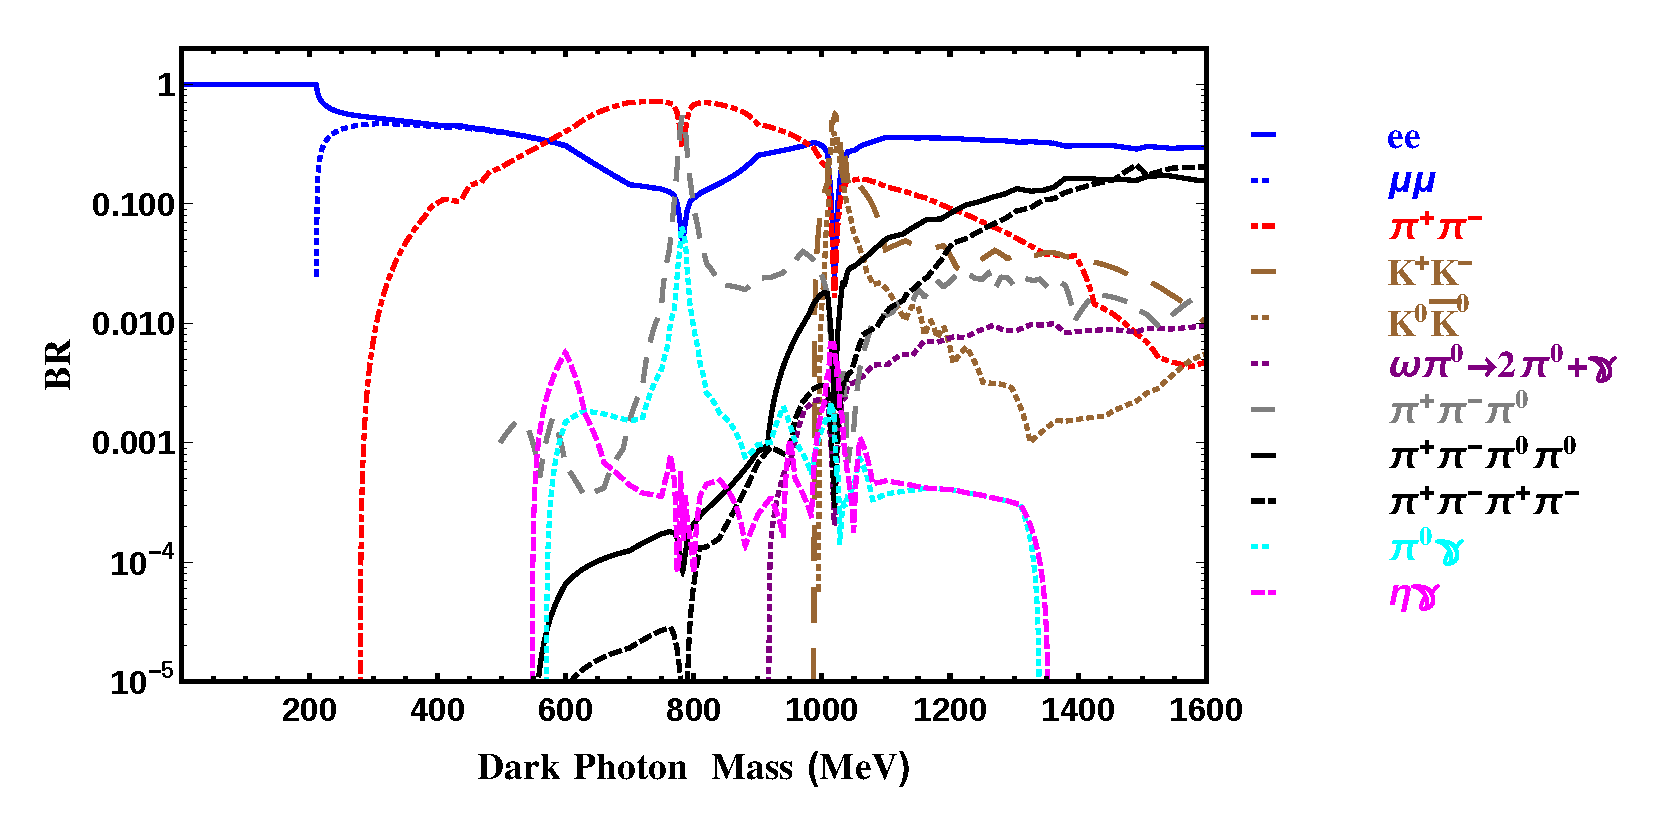
\includegraphics[width=\textwidth]{motivation/figs/darkphoton-BR-1-3000-LOG}
    \caption{Distribution of reconstructed invariant mass of M{\o}ller pairs, with a fit showing the mass resolution.}
    \label{fig:moller_mres}
\end{figure}

\begin{figure}[ht]
%    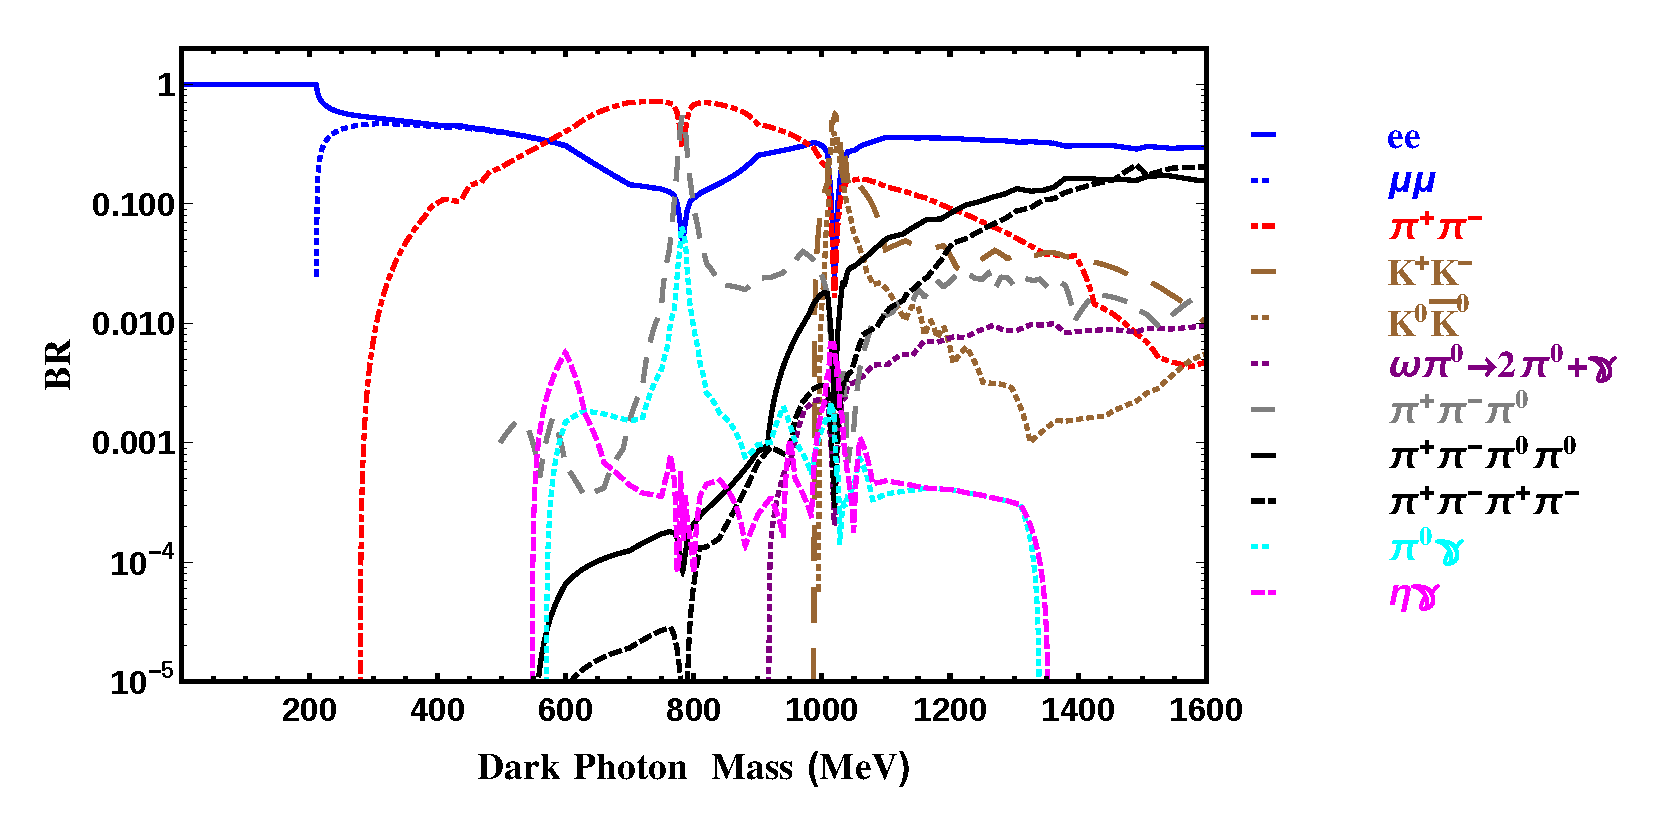
\includegraphics[width=\textwidth]{motivation/figs/darkphoton-BR-1-3000-LOG}
    \caption{Mass resolution from Monte Carlo of heavy photon decays, compared to mass resolution from M{\o}ller pairs.}
    \label{fig:mres_datamc}
\end{figure}

\subsection{Estimating the Signal Distribution}
\label{sec:signal_shape}
The signal distribution is as follows, where each term can depend on $m_{A'}$ and $\epsilon^2$:
\begin{equation}
S(z) = (N_{A'}\epsilon_{reco}(z_{target}))\frac{e^{\frac{z_{target}-z}{\gamma c \tau}}}{\gamma c \tau}\frac{\epsilon_{reco}(z)}{\epsilon_{reco}(z_{target})}
\end{equation}
$N_{A'}$ is the number of heavy photons produced in the target.
The exponential function is the distribution of decays along $z$, and is normalized to 1.
$\epsilon_{reco}(z)$ is the efficiency to detect and reconstruct an $e^+e^-$ pair produced at a given $z$.
In principle, this distribution should be smeared by $\sigma_z$, the resolution of the vertex position: this is not done since the signal distribution varies slowly on the scale of $\sigma_z$ (which is 3-6 mm, depending on $m$).

\subsubsection{Production Rate and Radiative Fraction}

$N_{A'}\epsilon_{reco}(z_{target})$ is estimated using data and Equation \ref{eq:production}, which shows that $N_{A'}$ is linked to $\frac{\mathrm{d}N_{rad}}{\mathrm{d}m}$, the number of radiative tridents produced with masses around $m_{A'}$.
The data gives $\frac{\mathrm{d}N_{e^+e^-}}{\mathrm{d}m}\epsilon_{reco}(z_{target})$, the number of $e^+e^-$ pairs produced and detected in a mass window around $m_{A'}$; some fraction of these are radiative tridents.
The fraction is estimated using Monte Carlo.

\begin{figure}[ht]
\begin{center}
    \includegraphics[width=0.35\textwidth,page=5,angle=-90]{vertexing/figs/frac}
    \includegraphics[width=0.35\textwidth,page=6,angle=-90]{vertexing/figs/frac}
\end{center}
    \caption{Left: rates of processes producing $e^+e^-$ pairs, with the sum in black. Right: the radiative fraction, which is calculated by dividing the black histogram by the red histogram.}
    \label{fig:radfrac}
\end{figure}

\subsubsection{Decay Length}
The decay length is calculated using Equation \ref{eq:lifetime}, which gives the lifetime $\tau$ for a given $m_{A'}$ and $\epsilon^2$.
The boost $\gamma$ equals $E_{beam}/m_{A'}$ if the heavy photon takes the full beam energy, but this is not completely accurate; in reality the average boost is slightly less than the maximum.

Monte Carlo is used to get the correct distribution of decay lengths.
The decay $z$ is plotted for an MC sample of heavy photons with mass $m_{A'}$ and an arbitrary lifetime, with the requirement that the heavy photon momentum be at least $0.8E_{beam}$ (matching the analysis cut), and fit with an exponential.
The decay constant of the exponential is compared to the $\gamma c \tau$ that would be expected from $\gamma=E_{beam}/m_{A'}$; this shows that the typical $\gamma$ is roughly $0.95E_{beam}/m_{A'}$.

\begin{figure}[ht]
\begin{center}
    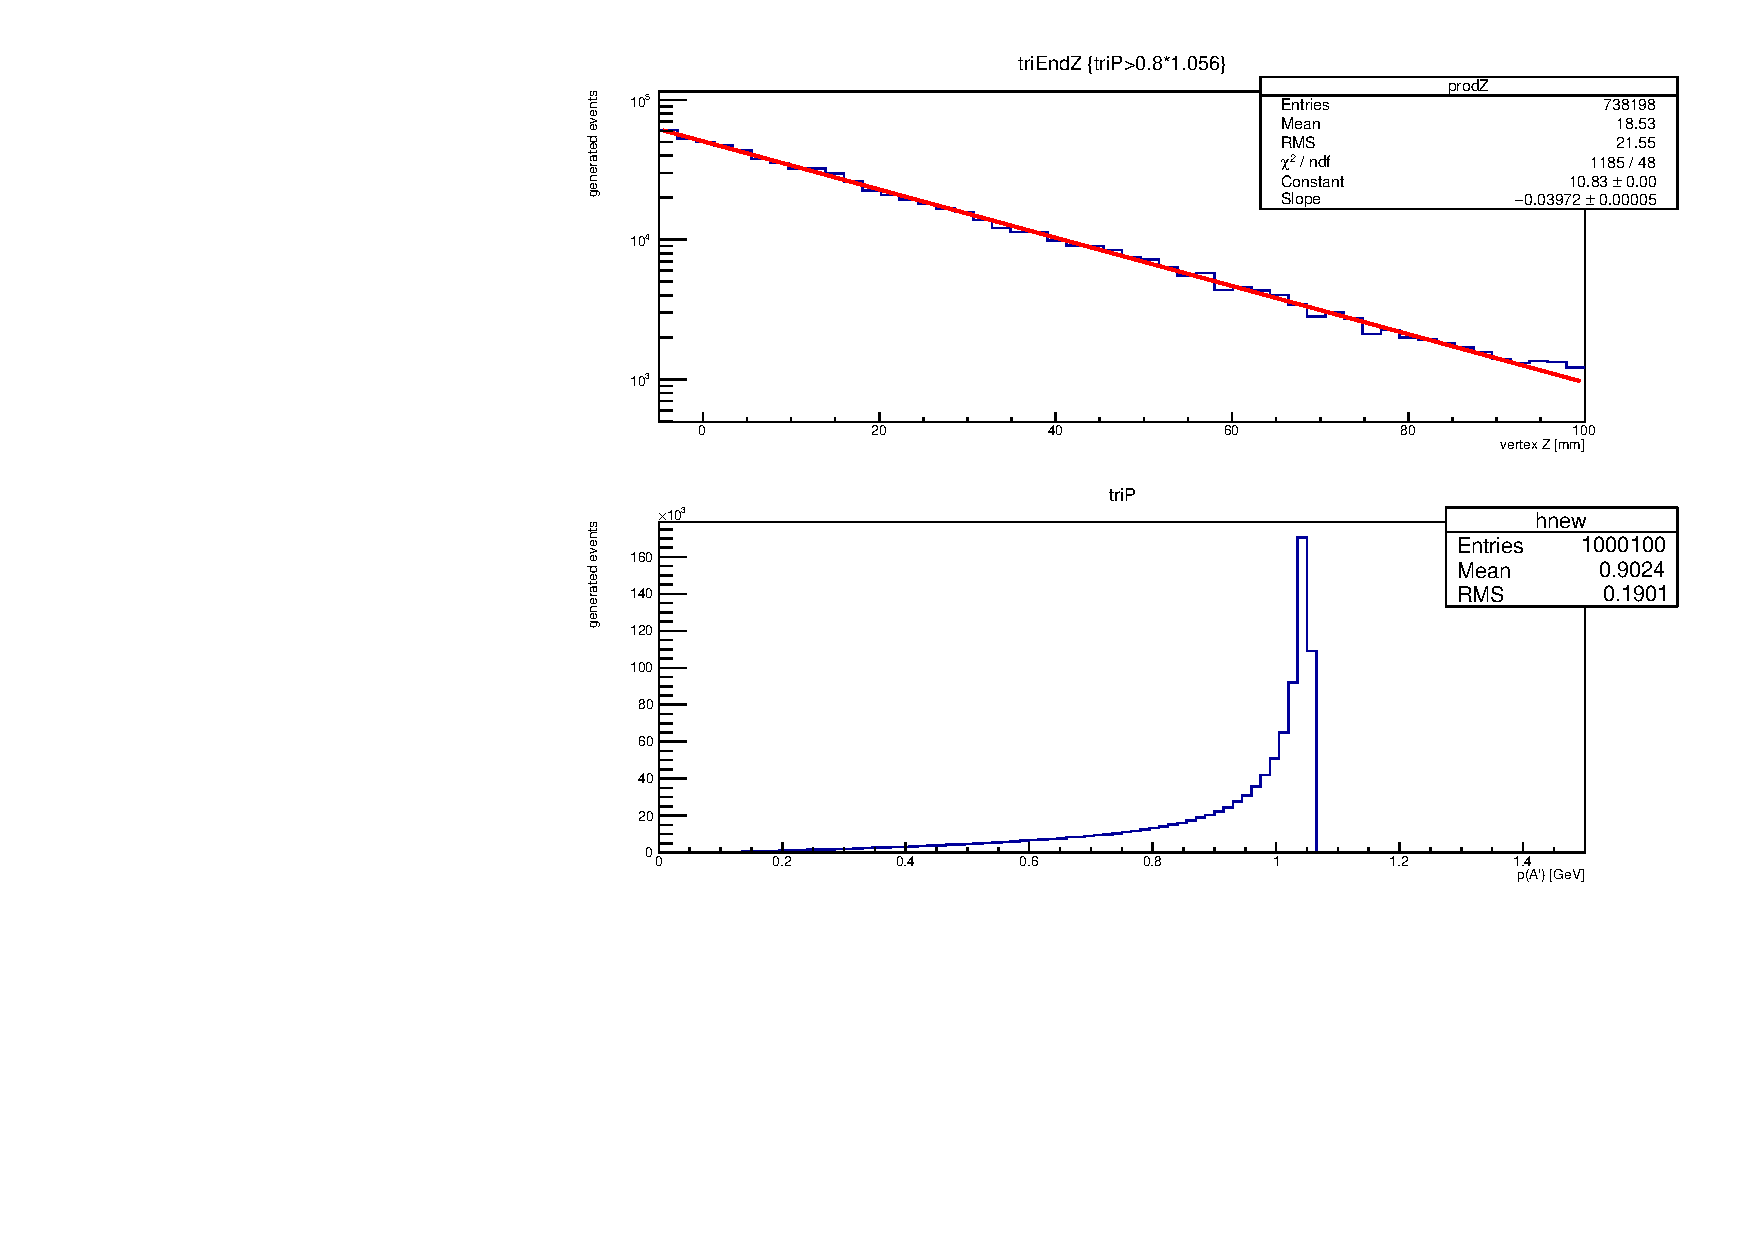
\includegraphics[width=0.7\textwidth,page=1,angle=-90]{vertexing/figs/acceptance_40}
\end{center}
    \caption{Top: distribution of decay $z$ for heavy photons ($m_{A'}=40$ MeV, $c\tau=1$ mm) carrying at least 80\% of the beam momentum. Bottom: the momentum distribution for the heavy photons.}
    \label{fig:decay_z_truth}
\end{figure}

\subsubsection{Efficiency}

The efficiency $\epsilon_{reco}$ for reconstructing a heavy photon decay depends on $m_{A'}$ and the decay $z$.
The measurement of the radiative trident rate implicitly includes a factor of $\epsilon_{reco}(m_{A'},z_{target})$, so Monte Carlo is only needed to estimate $\frac{\epsilon_{reco}(m_{A'},z)}{\epsilon_{reco}(m_{A'},z_{target})}$, the efficiency falloff as a function of vertex displacement.
This assumes that any detector-based inefficiencies not represented in the Monte Carlo are independent of $z$.

The efficiency falls off with $z$ because the further downstream the decay, the larger the opening angle in the Y-Z plane necessary to hit layer 1 of the tracker.
At some cutoff value of $z$ it is no longer possible for both the electron and the positron to hit layer 1; the efficiency starts to fall off well before that cutoff.
This effect is more severe for lower $m_{A'}$, where the opening angle is smaller.

The efficiency is measured using the Monte Carlo samples of generated and reconstructed heavy photons described in Section \ref{sec:ap_mc}.
For each $m_{A'}$, the distribution of decay $z$ is filled both for generated and reconstructed heavy photons.
The ratio of the two distributions gives $\epsilon_{reco}(m_{A'},z)$.
This is scaled so it equals 1 at $z=z_target$, and is fitted with a function of the form $\frac{\epsilon_{reco}(m_{A'},z)}{\epsilon_{reco}(m_{A'},z_{target})} \approx \exp(p_3 z^3 + p_2 z^2 + p_1 z + p_0)$.
The parameters $p_3$, $p_2$, $p_1$, and $p_0$ are fit with polynomials in $m_{A'}$: $p_0$ and $p_1$ are fit with first-order polynomials, and $p_2$ and $p_3$ are fit with third-order polynomials.

\begin{figure}[ht]
\begin{center}
    \includegraphics[width=0.7\textwidth,page=2,angle=-90]{vertexing/figs/acceptance_40}
\end{center}
    \caption{Top: distribution of decay $z$ for reconstructed heavy photons ($m_{A'}=40$ MeV, $c\tau=1$ mm). Bottom: efficiency curve $\frac{\epsilon_{reco}(m_{A'},z)}{\epsilon_{reco}(m_{A'},z_{target})}$, with fit.}
    \label{fig:eff_z}
\end{figure}

\subsection{Fitting the Background Distribution}
\label{sec:tails}
The background distribution consists of a Gaussian core and a non-Gaussian tail.
The width of the Gaussian core is set by multiple scattering and is well understood, but the tails extend much farther than the Gaussian.
For $z>z_{cut}$, the background distribution is dominated by the tails: $z_{cut}$ is typically at least $5\sigma_z$.

The tails of the vertex distribution mostly come from two sources: multiple scattering and mishits.

Multiple scattering is the source of the Gaussian core, and also plays a role in the tails.
If one of the particles scatters in the first layer of the tracker, the track parameters at the vertex will be shifted.
The distribution of scattering angles is Gaussian at small angles where the scattering process is approximated by a random walk, but at large angles, the distribution approaches the Rutherford scattering distribution, which is a power law.

If a particle scatters in the second (or later) layer of the tracker, the track may be shifted so that a layer-1 hit from a different particle is more in line with the hits from layers 2 on; the track fit will then add the wrong hit to the track, and the track parameters at the vertex will be shifted.

The background distribution is estimated from Monte Carlo.
This is necessary because if the background distribution were fit from the data, and there is actually a heavy photon signal in the data, the fit would be pulled so as to understate the size of the signal.
Comparisons of the background distribution in Monte Carlo and data show that the Monte Carlo accurately simulates the processes that create the tails.

The 2-dimensional vertex distribution from Monte Carlo is scanned in $m$, using the same mass cut that is used for the analysis.

The background distribution is fit with a 4-parameter piecewise function defined from a Gaussian and an exponential.
The Gaussian is defined with the usual parameters of mean and standard deviation.
The parameter $z_{tail}$ defines the distance from the Gaussian's mean where the distribution transitions to the exponential.
The exponential is defined in terms of a decay length, and its amplitude is fixed by the requirement that the function be continuous.
This function is similar to the ``GaussExp'' function described in \cite{search_cms_2015}, except GaussExp fixes the exponential's decay length by requiring that the function be continuously differentiable.
\begin{equation}
B(z;\bar{z},\sigma,b,l)=
\begin{cases}
e^{-\frac{(z-\bar{z})^2}{2\sigma^2}} &\text{if } z\le\bar{z}+b,\\
e^{-\frac{b^2}{2\sigma^2} - (z-\bar{z}-b)/l}  &\text{if } z\ge\bar{z}+b
\end{cases}
\end{equation}

The values of $b$ and $l$ found at each $m_{A'}$ are fitted to cubic polynomials in $m_{A'}$.
When estimating $B(z)$ for data, the values of $b$ and $l$ are fixed to the values found for Monte Carlo, but the Gaussian parameters are allowed to float.

\section{Setting Limits}


\subsection{Optimum Interval Method}
The method chosen for setting limits is the ``optimum interval'' method by Yellin \cite{yellin_finding_2002}.
This method was developed for direct detection experiments, and is intended for low-statistics experiments where the signal shape is known, but the backgrounds are not fully understood and there is the possibility of an unexpected background.

\begin{figure}[ht]
\begin{center}
    \includegraphics[width=0.35\textwidth,page=4,angle=-90]{vertexing/figs/toy_nothing}
    \includegraphics[width=0.35\textwidth,page=4,angle=-90]{vertexing/figs/toy_nosignal}
\end{center}
    \caption{Comparison of the optimum interval method with cut-and-count using Feldman-Cousins limits. The background (10000 events) has decay length 2, the signal has decay length 20, and the unexpected background (100 events) has decay length 5. Left plot is with only the expected background (no signal); right plot is with the unexpected background added (still no signal). The $z_{cut}$ for 0.5 expected background events is 19.8.}
    \label{fig:optimum_interval_demo}
\end{figure}


\begin{figure}[ht]
\begin{center}
    \includegraphics[width=0.7\textwidth,page=5,angle=-90]{vertexing/figs/golden_mres_output}
\end{center}
    \caption{Number of detectable heavy photon events expected past $z_{cut}$. The highest contour is at 0.3 events.}
    \label{fig:detectable}
\end{figure}

\begin{figure}[ht]
\begin{center}
    \includegraphics[width=0.7\textwidth,page=4,angle=-90]{vertexing/figs/golden_mres_output}
\end{center}
    \caption{90\% CL upper limit on the heavy photon production rate. A value of 1 would mean exclusion; the lowest contour on this plot is 200.}
    \label{fig:upper_limit}
\end{figure}
